\documentclass[11pt]{lecturenotes}

\newcommand{\code}[1]{\texttt{#1}}

\newcommand{\objExplainPrinciples}{\item explain the principles of survey design including question design, sampling, statistical inference, and sources of error}
\newcommand{\objDevelopQuestions}{\item explain the principles of survey design including question design, sampling, statistical inference, and sources of error}
\newcommand{\objAdvocate}{\item advocate for inclusion of measures on surveys using a scientific justification}
\newcommand{\objDataManagement}{\item conduct basic data management tasks and descriptive analysis in \textsf{R}}


\title{Populations, Frames, and Coverage}
\author{Michael Bader}
\week{3}
\lesson{1}
\coursenumber{SOCY 625}
\coursetitle{Practicum in Sociological Research}


\begin{document}
\maketitle

\begin{objectives}{
\item Define coverage, coverage error, clustering, and duplication
\item Describe methods of conducting a probability sample from a frame
\item Explain why we use sampling weights and how they are applied in a simple stratified sample}{
\objExplainPrinciples
}
\end{objectives}

\section[10]{Review Inference}

\section[]{Coverage \& Coverage Error}

\subsection[20]{Coverage Error}

\concept{undercoverage}{extent of target population \emph{missed} by sampling frame}

\concept{Ineligible Units}{units included in the sampling frame that are not part of the target population}

In general we worry most in our sample design about undercoverage. 

We can screen out ineligible units if necessary. It's costly to do so, and the opportunity cost of screening out those ineligible units will reduce our sample of eligible units, so it creates a problem in \emph{cost-effectiveness}. 

Missing units, however, is a bigger problem. We worry that we do not represent the true population to which we want to make claims about our sample. Remember that the benefit of survey research comes from the fact that we can say something about \emph{populations} if our sample is well designed. 

If it isn't, we don't have much to stand on because the questions we ask are generally not that good at getting at processes or explaining \emph{how} $x$ causes $y$. 

\textbf{Formal definition}

\slide\[
\overline{Y_c} - \overline{Y} = \frac{U}{N}\left(\overline{Y_c} - \overline{Y_u}\right)
\]

\begin{description}[noitemsep]
\item[$\overline{Y_c}$] Mean of the \emph{covered} population
\item[$\overline{Y}$] True underlying mean of the target population
\item[$U,N$] Number of uncovered units; total population of frame
\item[$\overline{Y_u}$] Mean of the \emph{uncovered} population
\end{description}

Left-hand side of the equation is the definition of error. The observed values (our mean from respondents) minus the true underlying value in the target population. 

On the right-hand side, the error is equal to: 1) the fraction of the population that's not covered in our sample and 2) the difference in means between the mean of the people in the target population covered in the sample minus the mean of the people in target population not sampled. 

What is the coverage error if the people from the target population that we do not sample is the same as the people we do sample [think, pair, share]?$\longrightarrow$0

In this case the coverage error would be \emph{unbiased}. Our estimate of the mean would not be any different if we had covered the portion of the target population that we had missed. 

Let's look at a couple of examples to show what all of this means. Let's assume that we have a target population of 100 units. 

\begin{center}
\includegraphics[scale=1]{../images/noCoverageError.pdf}
\end{center}

\slide This design might get panned because it has such low coverage rate. But, at least on this dimension of $Y$, the sampling frame has \emph{unbiased} undercoverage. 

\begin{center}
\includegraphics[scale=1]{../images/highCoverageError.pdf}
\end{center}

\slide This image reflects the ``Dewey Defeats Truman'' phenomenon. We have a large sample, but the sample is so badly biased that we do not actually make the proper inference about the population.

The second of these images is a much larger problem even thought it has lower undercoverage. 

\begin{center}
\includegraphics[scale=1]{../images/highBiasedCoverage.pdf}
\end{center}

\slide Here, our undercoverage is biased (the mean equals zero versus a true underlying mean of 8), but the amount of undercoverage is so small that it doesn't matter much if the undercoverage is biased. 

It's important to remember that $\overline{Y}$, $\overline{Y_c}$, and $\overline{Y_u}$ are \emph{unobserved}. We do not actually know what they are, and one of the biggest problems that we come across is not knowing whether we missed some major part of the population. 


\section{Probability Samples}
\slide
\concept{probability sample}{a sample taken using some form of randomization to select elements from the sample frame}

Inference to target populations \emph{requires} a probability sample of the population such that every unit has a \emph{non-zero probability} of being sampled. If a unit in the target population has no probability of being selected, then we cannot infer anything about that member based on our sample. And, if some members of the target population cannot be included in our survey, then we cannot generalize our results, or we cannot (correctly) infer the true value in the population. 

\subsection[5]{Simple Random Samples}
The easiest way to create a probability sample is what we call a simple random sample. 

\slide
\concept{simple random sample}{every element in a frame has an equal probability of selection into the sample}

\slide
We start, for example, by creating a list of all units in our sampling frame. We figure out how big we want our sample to be; figure out what proportion of the total sampling frame that number represents; then we select every $n$th unit from the frame. 

Let's say that we want to take a sample of rooms at a university dorm. In this dorm, there are eight floors with eight rooms on each. 

Let's pause for a second$\ldots$

What is our target population?$\longrightarrow$students living in the dorm

What is the sampling frame?$\longrightarrow$list of dorm rooms

Let's suppose that we want to take a 1/5 sample. We need to start at a random spot on the list (otherwise we would always pick the first unit, which might bias us). A simple random sample will randomly select every fifth unit on the list. Because we started at a random number, then every room had a \emph{chance} to be selected. 

\begin{center}
\slide
\small
\begin{minipage}{.4\textwidth}
\begin{tabular}{lr}
\multicolumn{2}{l}{\textbf{Random start = 2}} \\
\multicolumn{2}{l}{\textbf{Sample prop.\ 1/5}} \\
\textbf{Room \#} & \textbf{Selected?} \\ \toprule
101 & \\
102 & Y \\
103 & \\
104 & \\ 
105 & \\
106 & \\ 
107 &Y  \\
108 & \\
201 & \\
202 & \\
203 & \\
204 &Y \\ 
205 & \\
206 & \\ 
207 & \\
208 &\\ \bottomrule
\end{tabular}
\end{minipage}\begin{minipage}{.4\textwidth}
\begin{tabular}{lr}
\multicolumn{2}{l}{} \\
\multicolumn{2}{l}{} \\
\textbf{Room \#} & \textbf{Selected?} \\ \toprule
701 & \\
702 &  \\
703 & \\
704 &Y  \\ 
705 & \\
706 & \\ 
707 & \\
708 &\\
801 & Y \\
802 &  \\
803 & \\
804 & \\ 
805 & \\
806 & Y \\ 
807 & \\
808 &\\ \bottomrule
\end{tabular}
\end{minipage}
\end{center}
\normalsize

Out of the 64 units, we will have selected 13 for the sample (rooms 102, 107, 204, 301, 306, 403, 408, 505, 602, 607, 704, 801, 806)





\subsection[20]{Area Probability Samples}
Many times, we cannot feasibly create a sampling frame from which we can draw elements for an entire population. In the DC Area Survey, for example, we want to be able to say something about the 3,045,103 people 18 and over who live in the District and the bordering jurisdictions. There is no way that we can create a list of all 3,045,103 people. 

Instead, we might want to sample neighborhoods and then sample people from within those neighborhoods. This is called an area probability sample.

\slide
{\centering 
Sample places $\longrightarrow$ Sample housing units $\longrightarrow$ Sample people

}

Going back to the hypothetical example of the dorm. Let's say that we want our target population to be all undergraduates living in dorms on a university campus. We are also going to suppose that we are on a big campus. Trying to list every room in all of the dorms would be really time consuming. And, it would also be expensive to go to lots of different buildings rather than concentrating our effort in a couple. 

Let's say that we have the given set of dorms where the units (rooms) are known (but the room numbers are not): 

\slide
\begin{tabular}{lr}
\textbf{Building} & \textbf{Pop.} \\ \toprule
Dorm 1 & 64 \\
Dorm 2 & 64 \\
Dorm 3 & 64 \\
Dorm 4 & 200 \\
Dorm 5 & 200 \\
Dorm 6 & 400 \\
Dorm 8 & 400 \\
Dorm 9 & 400 \\
Dorm 10 & 8 \\ \bottomrule
\end{tabular}

We could draw a simple random sample of the dorms, let's say four. What if we drew Dorms 1, 2, 3, and 10. We would end up with low coverage (and likely a biased sampling frame because we would end up with only residents of small dorms). What we could do is sample by size of dorm. We could say that we could do two of the 64-unit dorms, and only one of the 200 and one of the 400. Based on a random sample within these clusters, we end up with: 

\slide
\begin{tabular}{lrr}
\textbf{Building} & \textbf{Pop.} & \textbf{Sampled?} \\ \toprule
Dorm 1 & 64 & \\
Dorm 2 & 64 & Y\\
Dorm 3 & 64 & Y \\ \midrule
Dorm 4 & 200& Y  \\
Dorm 5 & 200 & \\ \midrule
Dorm 6 & 400 & \\
Dorm 8 & 400 & Y \\
Dorm 9 & 400 & \\ \midrule
Dorm 10 & 8 & Y\\ \bottomrule
\end{tabular}

Now, we would try to enumerate the rooms in each of the selected dorms and draw a simple random sample from those dorms. This would be an example of an area probability sample. 

\textbf{Iraq Mortality Lancet Article}


For the DCAS, we will sample neighborhoods, which we will define as Census tracts, then get a list of addresses in those neighborhoods to mail the survey, and finally we will ask people to respond to the survey
{\centering
DCAS:\\
Sample nhoods $\longrightarrow$ Sample addresses $\longrightarrow$ Sample people

}






\subsection[20]{Sample Weights}


\subsection[10]{Sources of Error}

\slide
\concept{clustering}{multiple elements of the target population are represented by the same frame element (p.\ 77)}

What to do about clustering? 
\begin{enumerate}[nolistsep]
\item Interview all eligible people within a unit of the sampling frame (e.g., have all adults answer questions)
\begin{itemize}
\item May be difficult to get everyone
\item First respondents within cluster might tell later respondents about the survey and affect the answers of those who take it later
\item Can't determine sample size, and it might expand quickly
\end{itemize}
\item Sample eligible people within a unit of the sampling frame (e.g., select one adult in a household)
\begin{itemize}
\item Next\slash Last birthday method
\item Kish table

\slide
\begin{center}
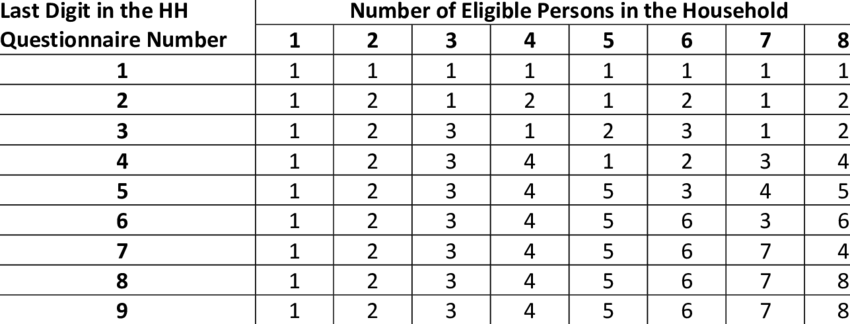
\includegraphics[scale=.9]{../images/Table-2-The-ILO-Modified-Kish-Grid.png}
\end{center}
\item Both methods will need to compensate for the \emph{within-cluster} probability of selection
\end{itemize}
\end{enumerate}

\slide
\concept{Duplication}{a single target population element is associated with multiple frame elements (p.\ 79)}

\end{document}
